\documentclass[10pt]{article}
\usepackage{mathtools}
\usepackage[margin=1.25in]{geometry}
\newcommand{\tab}[1]{\hspace{.05\textwidth}\rlap{#1}}
\begin{document}
\vspace*{\fill}
\begin{Huge}
\begin{center}
Ayush Jain (UNI : aj2672)\\
COMS W4180 Network Security\\
Written Assignment 1\\
\end{center}
\end{Huge}
\vspace*{\fill}
\newpage
\section{Problem 1}
\textbf{a)} Since UDP prefers speed over reliability, it may lead to packet loss and/or reordering. In such a situation \textbf{CTR} mode should be preferred because it provides for random read access(decryption of a particular cipher text does not depend on the previous one) and both encryption and decryption is parallelizable.\\\\
\textbf{b)} \textbf{CBC} should be used here because the message is small and hence can be padded with extra digits in the beginning. In that way, the decryption becomes independent of the IV used and can be easily decrypted.\\\\
\textbf{c)} Again, \textbf{CTR} should be used here as well. It is strong in terms of security and is parallelizable in encryption and decryption.\\\\
\textbf{d) EME} should be used for this use case. This is because it is more reliable as compared to XTS and CMC in terms of security. It is a bit slower as it requires two fold encryption, but at the same time it is parallelizable which can be a plus for distributed log files.
\section{Problem 2}
In the study, the set of collected keys were partitioned into different clusters shared the same RSA modulus. Out of about 6 million certificates collected about 200k certificates contain RSA modulus that is shared with another certificate.\\\\
We know that moduli that share one prime factor result in complete loss of security for all moduli involved. This means that two out of every one thousand RSA moduli that were collected offer no security at all. \\\\
This puts into question the assumption that different random choices are made each time keys are generated. The paper also concludes that generating keys in the real world for “multiple-secrets” cryptosystems such as RSA is significantly riskier than for “single-secret” ones such as ElGamal or (EC)DSA which are based on Diffie-Hellman.
\section{Problem 3}
\textbf{a)} The steps to encrypt and sign a file are:
\begin{enumerate}
\item Using the public key algorithm P and private key privkey and public key pubkey, compute and exchange the secret K.
\item use hash function H to hash the message.
\item use block cipher B and key K to encrypt the file and produce the digital signature.\\
\end{enumerate}
\textbf{b)} The steps to verify the signature on the file are:
\begin{enumerate}
\item Decrypt signature using secret key K and block cipher B.
\item hash original data using H
\item compare results from the two.
\end{enumerate}
\section{Problem 4}
Following is the code snippet used to compute the shared key using Diffie-Hellman key exchange.
\begin{figure}[ht!]
\centering
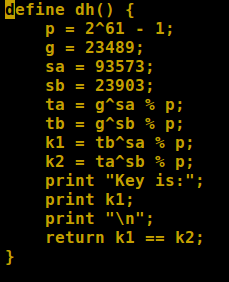
\includegraphics[width=50mm]{code.jpg}
\end{figure}\\
The output produced using the above code was:
\begin{figure}[ht!]
\centering
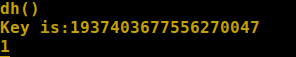
\includegraphics[width=50mm]{output.png}
\end{figure}\\
The dh() is the function call, followed by the key computed. 1 in the last line proves that the two keys were equal.
\section{Problem 5}
When selecting a new algorithm, the simplicity of the algorithm reduces implementation errors. It also makes sure that the costs such as power consumption, number of hardware gates and execution time is minimal.\\
\section{Problem 6}
\textbf{a)} It is necessary to start devising algorithms for quantum computing because it usually takes years, close to a decade to devise and accept new algorithms. This is because of the time and thoroughness that goes into testing the algorithm and pronouncing it safe. At the same time, elimination of existing algorithms also takes an equivalent amount of time.
So if we do not start coming up with quantum safe algorithms, current ones dependent on mathematically hard problems will still be in use when quantum computers come around. And with quantum computers cracking such algorithms will not be a problem because of the speed of such computers.\\\\\\
\textbf{b)} Diffie-Hellman is a bigger problem and needs to be replaced with quantum safe algorithm. This is because the mathematical hard problem on which DH algorithm depends upon can be easily solved by a sufficiently large quantum computer. AES can still be effective in presence of quantum safe computers if we increase the key size.\\
\section{Problem 7}
In my view, this can be a problem, because measuring the time can be an effective hint to the range in which the shared secret lies. The algorithm are based on mathematical hardness of the problem of checking each key. However, if we know the approximate range of our key, the test range decreases and hence figuring out the key would be much simpler, thus posing a security risk.
\end{document}